% !Mode:: "TeX:UTF-8"
\def\usewhat{pdflatex}                               % 定义编译方式 dvipdfmx 或者 pdflatex,默认为 dvipdfmx
                                                     % 方式编译,如果需要修改,只需改变花括号中的内容即可。
%\documentclass[12pt,openany,oneside]{book}

\documentclass[a4paper, 11pt]{article}                                                   % 本科生毕业论文通常采用单页排版
\usepackage{pdfpages}
\usepackage{float}
\usepackage{wrapfig}

%\usepackage{indentfirst}

%\usepackage{graphicx}
%\usepackage{caption}
%\usepackage{subcaption}
%\usepackage{subfigure}

%\makeatletter
%\let\c@subfigure\relax
%\let\l@subfigure\relax
%\makeatother

%\usepackage{epstopdf}


% !Mode:: "TeX:UTF-8"
%  Authors: 张井   Jing Zhang: prayever@gmail.com     天津大学2010 级管理与经济学部信息管理与信息系统专业硕士生
%           余蓝涛 Lantao Yu: lantaoyu1991@gmail.com  天津大学2008 级精密仪器与光电子工程学院测控技术与仪器专业本科生

%%%%%%%%%% Package %%%%%%%%%%%%
\usepackage{graphicx}                       % 支持插图处理
\usepackage[a4paper,text={146.4true mm,239.2 true mm},top= 26.2true mm,left=31.8 true mm,head=6true mm,headsep=6.5true mm,foot=16.5true mm]{geometry}
                                            % 支持版面尺寸设置
\usepackage[squaren]{SIunits}               % 支持国际标准单位

\usepackage{titlesec}                       % 控制标题的宏包
\usepackage{titletoc}                       % 控制目录的宏包
\usepackage{fancyhdr}                       % fancyhdr宏包 支持页眉和页脚的相关定义
\usepackage[UTF8]{ctex}                     % 支持中文显示
\usepackage{CJKpunct}                       % 精细调整中文的标点符号
\usepackage{color}                          % 支持彩色
\usepackage{amsmath}                        % AMSLaTeX宏包 用来排出更加漂亮的公式
\usepackage{amssymb}                        % 数学符号生成命令
\usepackage[below]{placeins}    %允许上一个section的浮动图形出现在下一个section的开始部分,还提供\FloatBarrier命令,使所有未处理的浮动图形立即被处理
\usepackage{multirow}                       % 使用Multirow宏包,使得表格可以合并多个row格
\usepackage{booktabs}                       % 表格,横的粗线;\specialrule{1pt}{0pt}{0pt}
\usepackage{longtable}                      % 支持跨页的表格。
\usepackage{tabularx}                       % 自动设置表格的列宽

%\makeatletter
%\let\c@subfigure\relax
%\makeatother

\usepackage{subfigure}                      % 支持子图 %centerlast 设置最后一行是否居中
\usepackage[subfigure]{ccaption}            % 支持子图的中文标题
\usepackage[sort&compress,numbers]{natbib}  % 支持引用缩写的宏包
\usepackage{enumitem}                       % 使用enumitem宏包,改变列表项的格式
\usepackage{calc}                           % 长度可以用+ - * / 进行计算
\usepackage{txfonts}                        % 字体宏包
\usepackage{bm}                             % 处理数学公式中的黑斜体的宏包
\usepackage[amsmath,thmmarks,hyperref]{ntheorem}  % 定理类环境宏包,其中 amsmath 选项用来兼容 AMS LaTeX 的宏包
\usepackage{CJKnumb}                        % 提供将阿拉伯数字转换成中文数字的命令
\usepackage{indentfirst}                    % 首行缩进宏包
\usepackage{CJKutf8}                        % 用在UTF8编码环境下,它可以自动调用CJK,同时针对UTF8编码作了设置
%\usepackage{hypbmsec}                      % 用来控制书签中标题显示内容
\newcommand{\tabincell}[2]{\begin{tabular}{@{}#1@{}}#2\end{tabular}}
\usepackage{xcolor}
%支持代码环境
\usepackage{listings}
\lstset{numbers=left,
language=[ANSI]{C},
numberstyle=\tiny,
extendedchars=false,
showstringspaces=false,
breakatwhitespace=false,
breaklines=true,
captionpos=b,
keywordstyle=\color{blue!70},
commentstyle=\color{red!50!green!50!blue!50},
frame=shadowbox,
rulesepcolor=\color{red!20!green!20!blue!20}
}
%支持算法环境
\usepackage[boxed,ruled,lined]{algorithm2e}
\usepackage{algorithmic}

\usepackage{array}
\newcommand{\PreserveBackslash}[1]{\let\temp=\\#1\let\\=\temp}
\newcolumntype{C}[1]{>{\PreserveBackslash\centering}p{#1}}
\newcolumntype{R}[1]{>{\PreserveBackslash\raggedleft}p{#1}}
\newcolumntype{L}[1]{>{\PreserveBackslash\raggedright}p{#1}}

% 生成有书签的 pdf 及其生成方式。通常可以在 tjumain.tex 文件的第一行选择 pdflatex 或者是 dvipdfmx 编译手段。如果选择前者,则使用 pdflatex + pdflatex 编译; 如果选择后者,在编译的时候选择 latex + bibtex + latex + latex 编译。出现混淆的时候,系统会报错。
% 如果您的pdf制作中文书签有乱码使用如下命令,就可以解决了
\def\atemp{dvipdfmx}\ifx\atemp\usewhat
\usepackage[dvipdfmx,unicode,               % dvipdfmx 编译, 加入了中文复制,粘贴支持引擎。
            pdfstartview=FitH,
            bookmarksnumbered=true,
            bookmarksopen=true,
            colorlinks=false,
            pdfborder={0 0 1},
            citecolor=blue,
            linkcolor=red,
            anchorcolor=green,
            urlcolor=blue,
            breaklinks=true
            ]{hyperref}
\fi

\def\atemp{pdflatex}\ifx\atemp\usewhat
\usepackage{cmap}                           % pdflatex 编译时,可以生成可复制、粘贴的中文 PDF 文档, 缺点是在Windows上显示时效果不大好,字体发虚
\usepackage[pdftex,unicode,
            %CJKbookmarks=true,
            bookmarksnumbered=true,
            bookmarksopen=true,
            colorlinks=false,
            pdfborder={0 0 1},
            citecolor=blue,
            linkcolor=red,
            anchorcolor=green,
            urlcolor=blue,
            breaklinks=true
            ]{hyperref}
\fi
                                % 定义本文所使用宏包
\graphicspath{{figures/}}                            % 定义所有的 .eps 文件在 figures 子目录下
\begin{document}                                     % 开始全文

\begin{CJK*}{UTF8}{song}
\begin{center}

  \begin{figure}[h]
  \centering
  
\includegraphics[width=0.7\textwidth]{figures/ustc}
  \end{figure}

\vspace*{25pt}
{ \fontsize{20pt}{24pt}\selectfont{\textbf{“大学生创新训练计划”项目结题报告}}}

\vspace*{20pt}

\begin{center}
  \begin{tabular}{lclc}
    中文题目 &  \underline{基于SDN的云中大数据网络优化的研究} \\
    英\qquad 文& \underline{ Research of bigdata network optimization} \\
    题\qquad 目& \underline{based on SDN in cloud computing} \\
    学\qquad 院& \underline{信息学院} \\
    指导教师 &  \underline{张文逸} \\
    \end{tabular}
    \vspace*{50pt}
    \begin{tabular}{lclc}
    小组成员: \\
    姓\qquad 名& \underline{孟思尧} & 学\qquad 号 & \underline{PB12210076} \\
    姓\qquad 名& \underline{王笑霄} & 学\qquad 号 & \underline{PB12210100} \\
    姓\qquad 名& \underline{张广帅}  & 学\qquad 号 & \underline{PB12210080} \\
  \end{tabular}
\end{center}

  \vspace*{25pt}
  \today

\end{center}
\clearpage
\begin{center}
  { \fontsize{15pt}{18pt}\selectfont{\textbf{摘\qquad 要}}}
\end{center}

{ \fontsize{10pt}{15pt}\selectfont{\textbf{关键词:}}}云计算,大数据,SDN,HADOOP,网络优化
\clearpage
\begin{center}
  { \fontsize{15pt}{18pt}\selectfont{\textbf{ABSTRACT}}}
\end{center}

{ \fontsize{10pt}{15pt}\selectfont{\textbf{KEY WORDS:}}}Cloud computing,Bigdata,SDN,HADOOP,network optimization
\clearpage
\tableofcontents
%\part{问题阐述}
%\chapter{问题阐述}
\section{项目背景}
\subsection{项目的意义和关键问题}
大数据应用正深刻改变人们的生活,已经成为当前学术界、工业界的关注焦点。大数据应用开发云平台纷纷推出大数据计算框架。如Amazon的EC2,微软的Azure。虽然云平台上的大数据框架方便了第三方开发者和用户,但其性能上还存在较多问题,尤其是网络的问题。在2014 Daytona GraySort排序赛上,基于Spark的系统它使用了207个EC2 节点在23分钟内排序了100TB的数据而夺冠。而上届冠军Hadoop用了2100台Yahoo内置的机器,花了72分钟,这性能提升不言而喻!更重要的是这次比赛证实Shuffle真正的瓶颈在于网络。传统大数据网络架构是数据库服务器将应用服务器请求的数据通过网络传输到应用服务器上,处理后,将改写的数据再写回数据库服务器,而且处理过程中会出现大量的中间结果也需要网络传输。当数据量较大时,很可能堵塞网络。因而对于进一步提升大数据处理性能,研究云平台上大数据网络问题显得尤为重要。\\
\subsection{研究方向}
\begin{description}
  \item[软件定义网络(SDN)] 软件定义网络(SDN)是当前和未来网络研究的一个重要方向,通过将网络的数据转发层和逻辑控制层分离,提高了网络的灵活性和可编程性。可以在控制层面设计应用感知的控制策略,如网络接入、数据转发路由、流量工程等,从而提高应用的性能。因此,我们拟通过SDN来优化云平台上大数据框架的网络性能。
  \item[coflow调度] 考虑到当前数据中心用并行计算的框架处理大规模的数据,充分考虑数据流的相关性(coflow),设计调度算法
\end{description}
\section{项目平台的选择}
\subsection{Hadoop}
\subsubsection{为什么选择Hadoop}
数据并行计算框架很多,如:Mapreduce,Spark,Google Dataflow等等,我们为什么选择Hadoop?
首先,认识一下Hadoop,Hadoop是一种计算集群,它将数据分析的工作分配到多个集群节点上,从而并行处理数据。经过调研,Hadoop用于大数据处理,主要有如下几个优势:
\begin{description}
  \item[1、灵活的可扩展性] 要充分利用大数据最大的优势就需要实时或接近实时地对海量数据进行分析处理。大数据分析面临的一个巨大的难题是数据量的不断增加。而Hadoop集群的并行处理能力能明显提高分析速度,但随着要分析的数据量的增加,集群的处理能力会受到影响。Hadoop通过增加集群节点,可以线性地扩展集群以处理更大的数据集。另外,在集群负载下降时,也可以减少节点,以高效使用计算资源。所以Hadoop的弹性很好
  \item[2、Hadoop的设计适合大数据处理] 大数据一般都是分布广泛的并且是非结构化的。而Hadoop非常适合处理这类数据,因为Hadoop的mapreduce的计算框架工作原理是将数据拆分成片,并将每个“分片”分配到特定的集群节点上进行分析。数据不必均匀分布,因为每个数据分片都是在独立的集群节点上进行单独处理。
  \item[3、Hadoop成本低] Hadoop的软件是开源的,同时,Hadoop支持商用硬件,可以运行在一般商业机器构成的大型集群上,如:亚马逊弹性计算云(Amazon EC2)等,不必花费重金购买服务器级别的硬件设备。所以我们可以低成本的实现计算能力强大的Hadoop集群,性价比很高。
  \item[4、容错能力强] 在Hadoop集群进行大数据处理分析过程中,当一个数据分片发送到某个节点进行分析时,该数据在集群其它节点上会存有副本。通过备份的方式,即使一个节点发生故障,数据可以快速的恢复,继续进行分析处理。故障检测和自动恢复是Hadoop最初的设计目标,所以Hadoop很健壮。
\end{description}
由于Hadoop具有上述优势,使得Hadoop在学术界和工业界都大受欢迎。\\
\subsubsection{Mapreduce计算框架}
Mapreduce是什么?怎样完成大数据处理?\\
Hadoop的设计思路源于Google的GFS和MapReduce。它是一个开源软件框架,通过在集群计算机中使用MapReduce这个简单的编程模型,可编写和运行分布式应用程序处理大规模数据。

\begin{figure}[!htb]
    \centering
    \let\c@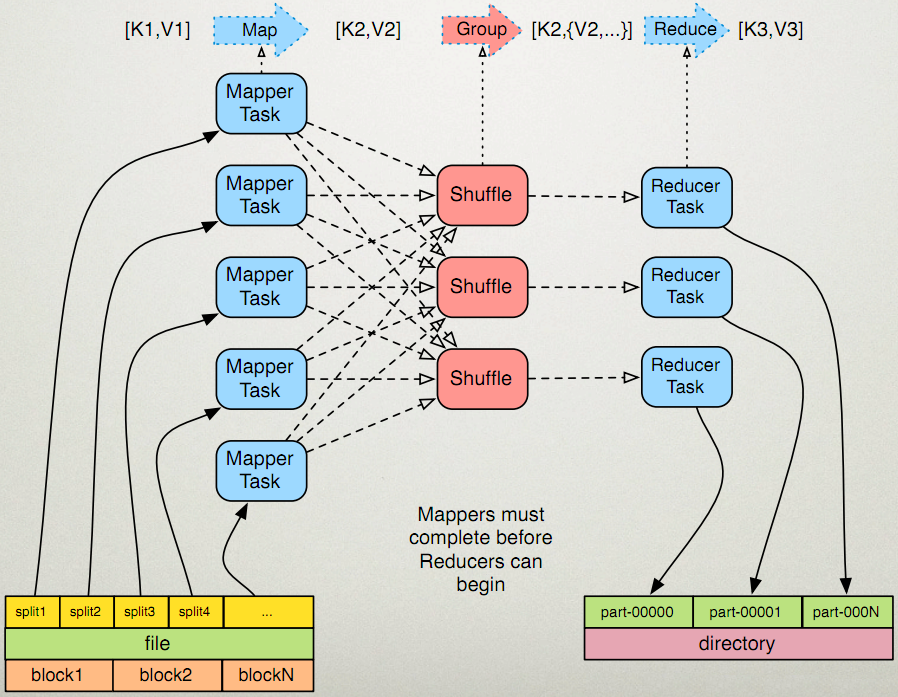
\includegraphics[height=2in]{mapreduce.png}\relax
    \caption{Mapreduce计算框架}
\end{figure}
MapReduce架构的大数据处理的操作流程如下:
\begin{enumerate}
  \item 首先调用MapReduce库的输入流模块,将输入文件分成M个数据片度,每个数据片段的大小可以通过可选的参数来控制。然后用户程序在机群中创建大量的程序副本。程序副本中包含一个特殊的master程序。其它的程序都是worker程序,由master分配任务。有M个Map任务和R个Reduce任务将被分配,master将一个Map任务或Reduce任务分配给一个空闲的worker。
  \item 被分配了map任务的worker程序读取相关的输入数据片段,从输入的数据片段中解析出key/value pair,然后把key/value pair传递给用户自定义的Map函数,由Map函数生成并输出的中间key/value pair,并缓存在内存中。
  \item 缓存中的key/value pair通过调用Partition模块分成R个区域,之后周期性的写入到本地磁盘上。缓存的key/value pair在本地磁盘上的存储位置将被传给master,由master负责把这些存储位置再传送给Reduce worker。
  \item 当Reduce worker程序接收到master程序发来的数据存储位置信息后,使用RPC从Map worker所在主机的磁盘上读取这些缓存数据。当Reduce worker读取了所有的中间数据后,通过对key进行排序后使得具有相同key值的数据聚合在一起。由于许多不同的key值会映射到相同的Reduce任务上,因此必须进行排序。如果中间数据太大无法在内存中完成排序,那么就要在外部进行排序。
  \item Reduce worker程序遍历排序后的中间数据,对于每一个唯一的中间key值,Reduce worker程序将这个key值和它相关的中间value值的集合传递给用户自定义的Reduce函数。Reduce函数的输出被追加到所属分区的输出文件。
  \item 当所有的Map和Reduce任务都完成之后,master唤醒用户程序。在这个时候,在用户程序里的对MapReduce调用才返回。在成功完成任务之后,MapReduce的输出存放在R个输出文件中(对应每个Reduce任务产生一个输出文件,文件名由用户指定)。一般情况下,用户不需要将这R个输出文件合并成一个文件–他们经常把这些文件作为另外一个MapReduce的输入,或者在另外一个可以处理多个分割文件的分布式应用中使用。
\end{enumerate}

\subsubsection{Shuffle阶段}
整体的Shuffle过程包含以下几个部分:Map端Shuffle、Sort阶段、Reduce端Shuffle。即是说:Shuffle 过程横跨 map 和 reduce 两端,中间包含 sort 阶段。 

\begin{figure}[!htb]
    \centering
    \let\c@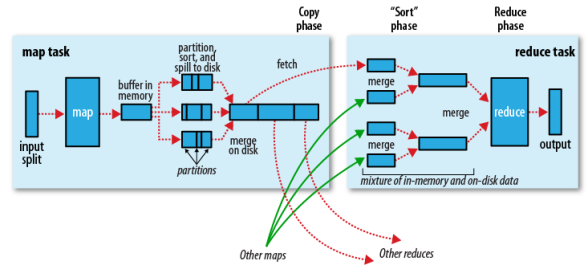
\includegraphics[height=2in]{shuffle.png}\relax
    \caption{shuffle阶段}
\end{figure}
 在Hadoop集群中,大部分map task与reduce task的执行是在不同的节点上,Reducer通过Http方式得到map阶段输出文件的分区,所以很多情况下Reduce 执行时需要跨节点去拉取其它节点上的map task结果。在Mapreduce的Shuffle阶段,如果集群正在运行的 job 有很多,而且需要跨节点拉取数据时,会产生大量的数据在网络中传输,对集群内部的网络资源消耗会很严重,尽可能地减少对带宽的不必要消耗,并且保证完整地从map task 端拉取数据到reduce端。\\

\subsection{SDN}
SDN(软件定义网络)利用OpenFlow协议,把路由器的控制平面(control plane)从数据平面(data plane)中分离出来,以软件方式实现。这个架构可以让网络管理员,在不改动硬件设备的前提下,通过集中式的控制器(Controller)以标准化的接口对各种网络设备进行管理和配置,那么这将为网络资源的设计、管理和使用提供更多的可能性,为控制网络流量提供了新的方法。\\
控制器作为SDN网络中的重要组成部分,我们选择Floodlight作为SDN控制器。因为Floodlight是目前主流的SDN控制器之一,它的稳定性、易用性已经得到SDN专业人士一致好评,由于其完全开源,这让SDN网络世界变得更加有活力。能集中地灵活控制SDN网络,为核心网络及应用创新提供了良好的扩展平台。\\
Floodlight控制器是一个企业级的,使用Java开发的OpenFlow协议的控制器。OpenFlow是一个由Open Networking Foundation (ONF)管理的开放标准。它定义了一种协议让远程控制器通过路由器可以修改网络设备的行为,使用定义良好的转发指令集。Floodlight被设计为同支持OpenFlow标准的设备(交换机,路由器,虚拟交换机)一起工作。\\
Floodlight controller模块为多数应用实现了一些通用的功能:

\begin{enumerate}
  \item 发现网络状态和事件(拓扑结构,设备,流量)
  \item 能够控制网络交换机(network switches)通信
  \item 管理floodlight模块,共享存储,线程,测试等资源
  \item 提供一个web界面和debug服务器(Python)
\end{enumerate}

\section{coflow相关知识介绍}
另外考虑到当前数据中心用并行计算的框架处理大规模的数据,有人提出了coflow的概念。coflow是一组相关的并行数据流的集合,coflow的完成时间由最后一条数据流的完成时间决定。

\begin{figure}[!htb]
    \centering
    \let\c@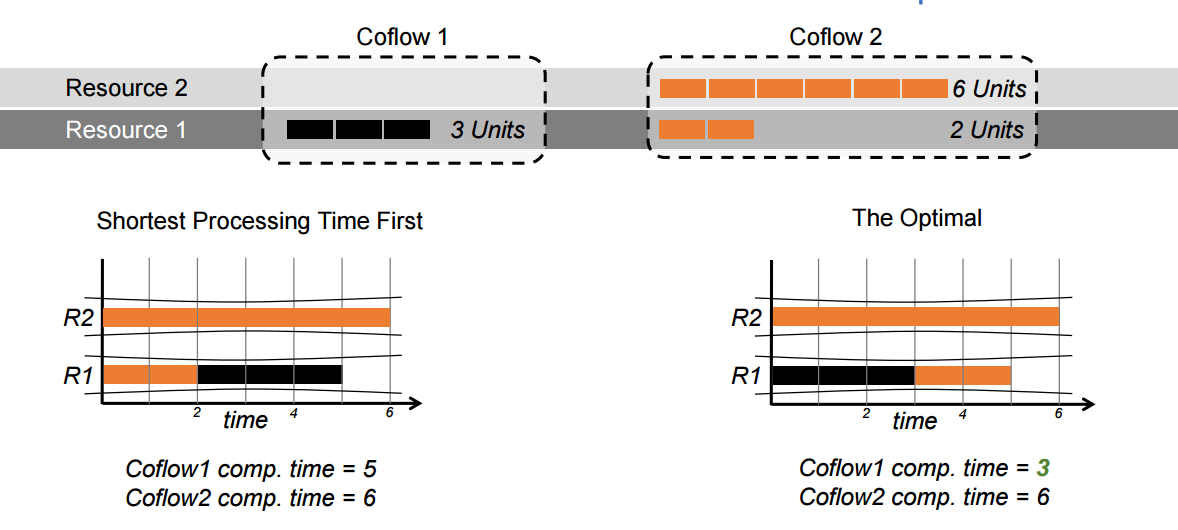
\includegraphics[height=2in]{coflow_cct.png}\relax
    \caption{coflow完成时间的比较}
\end{figure}
此处可详细说明一下这个例子\\
有人设计了varys来提高大数据处理过程中网络通信的性能,他们以最小化完成时间和满足deadline为目标实现了FIFO、SCF和SEBF等启发式算法。采用varys 仿真器coflowsim完成Facebook真实数据的调度测试。\\
coflow研究现状中存在的问题:
\begin{enumerate}
  \item 当前coflowsim中的调度策略都假设所有的flow都是同时出现,不太符合实际情况
  \item 当前的各种启发式算法都是在coflowsim中实现的,还没有用varys调度真实的Facebook数据流,
  \item 当前coflow的两层架构:inter-transfer负责多个transfer间的资源调度,intra-transfer负责一个transfer内的调度。inter-transfer策略主要是加权共享,并没有考虑多个flow间的dependency。
\end{enumerate}

\section{项目内容}
\subsection{实验环境}
\begin{figure}[!htb]
    \centering
    \let\c@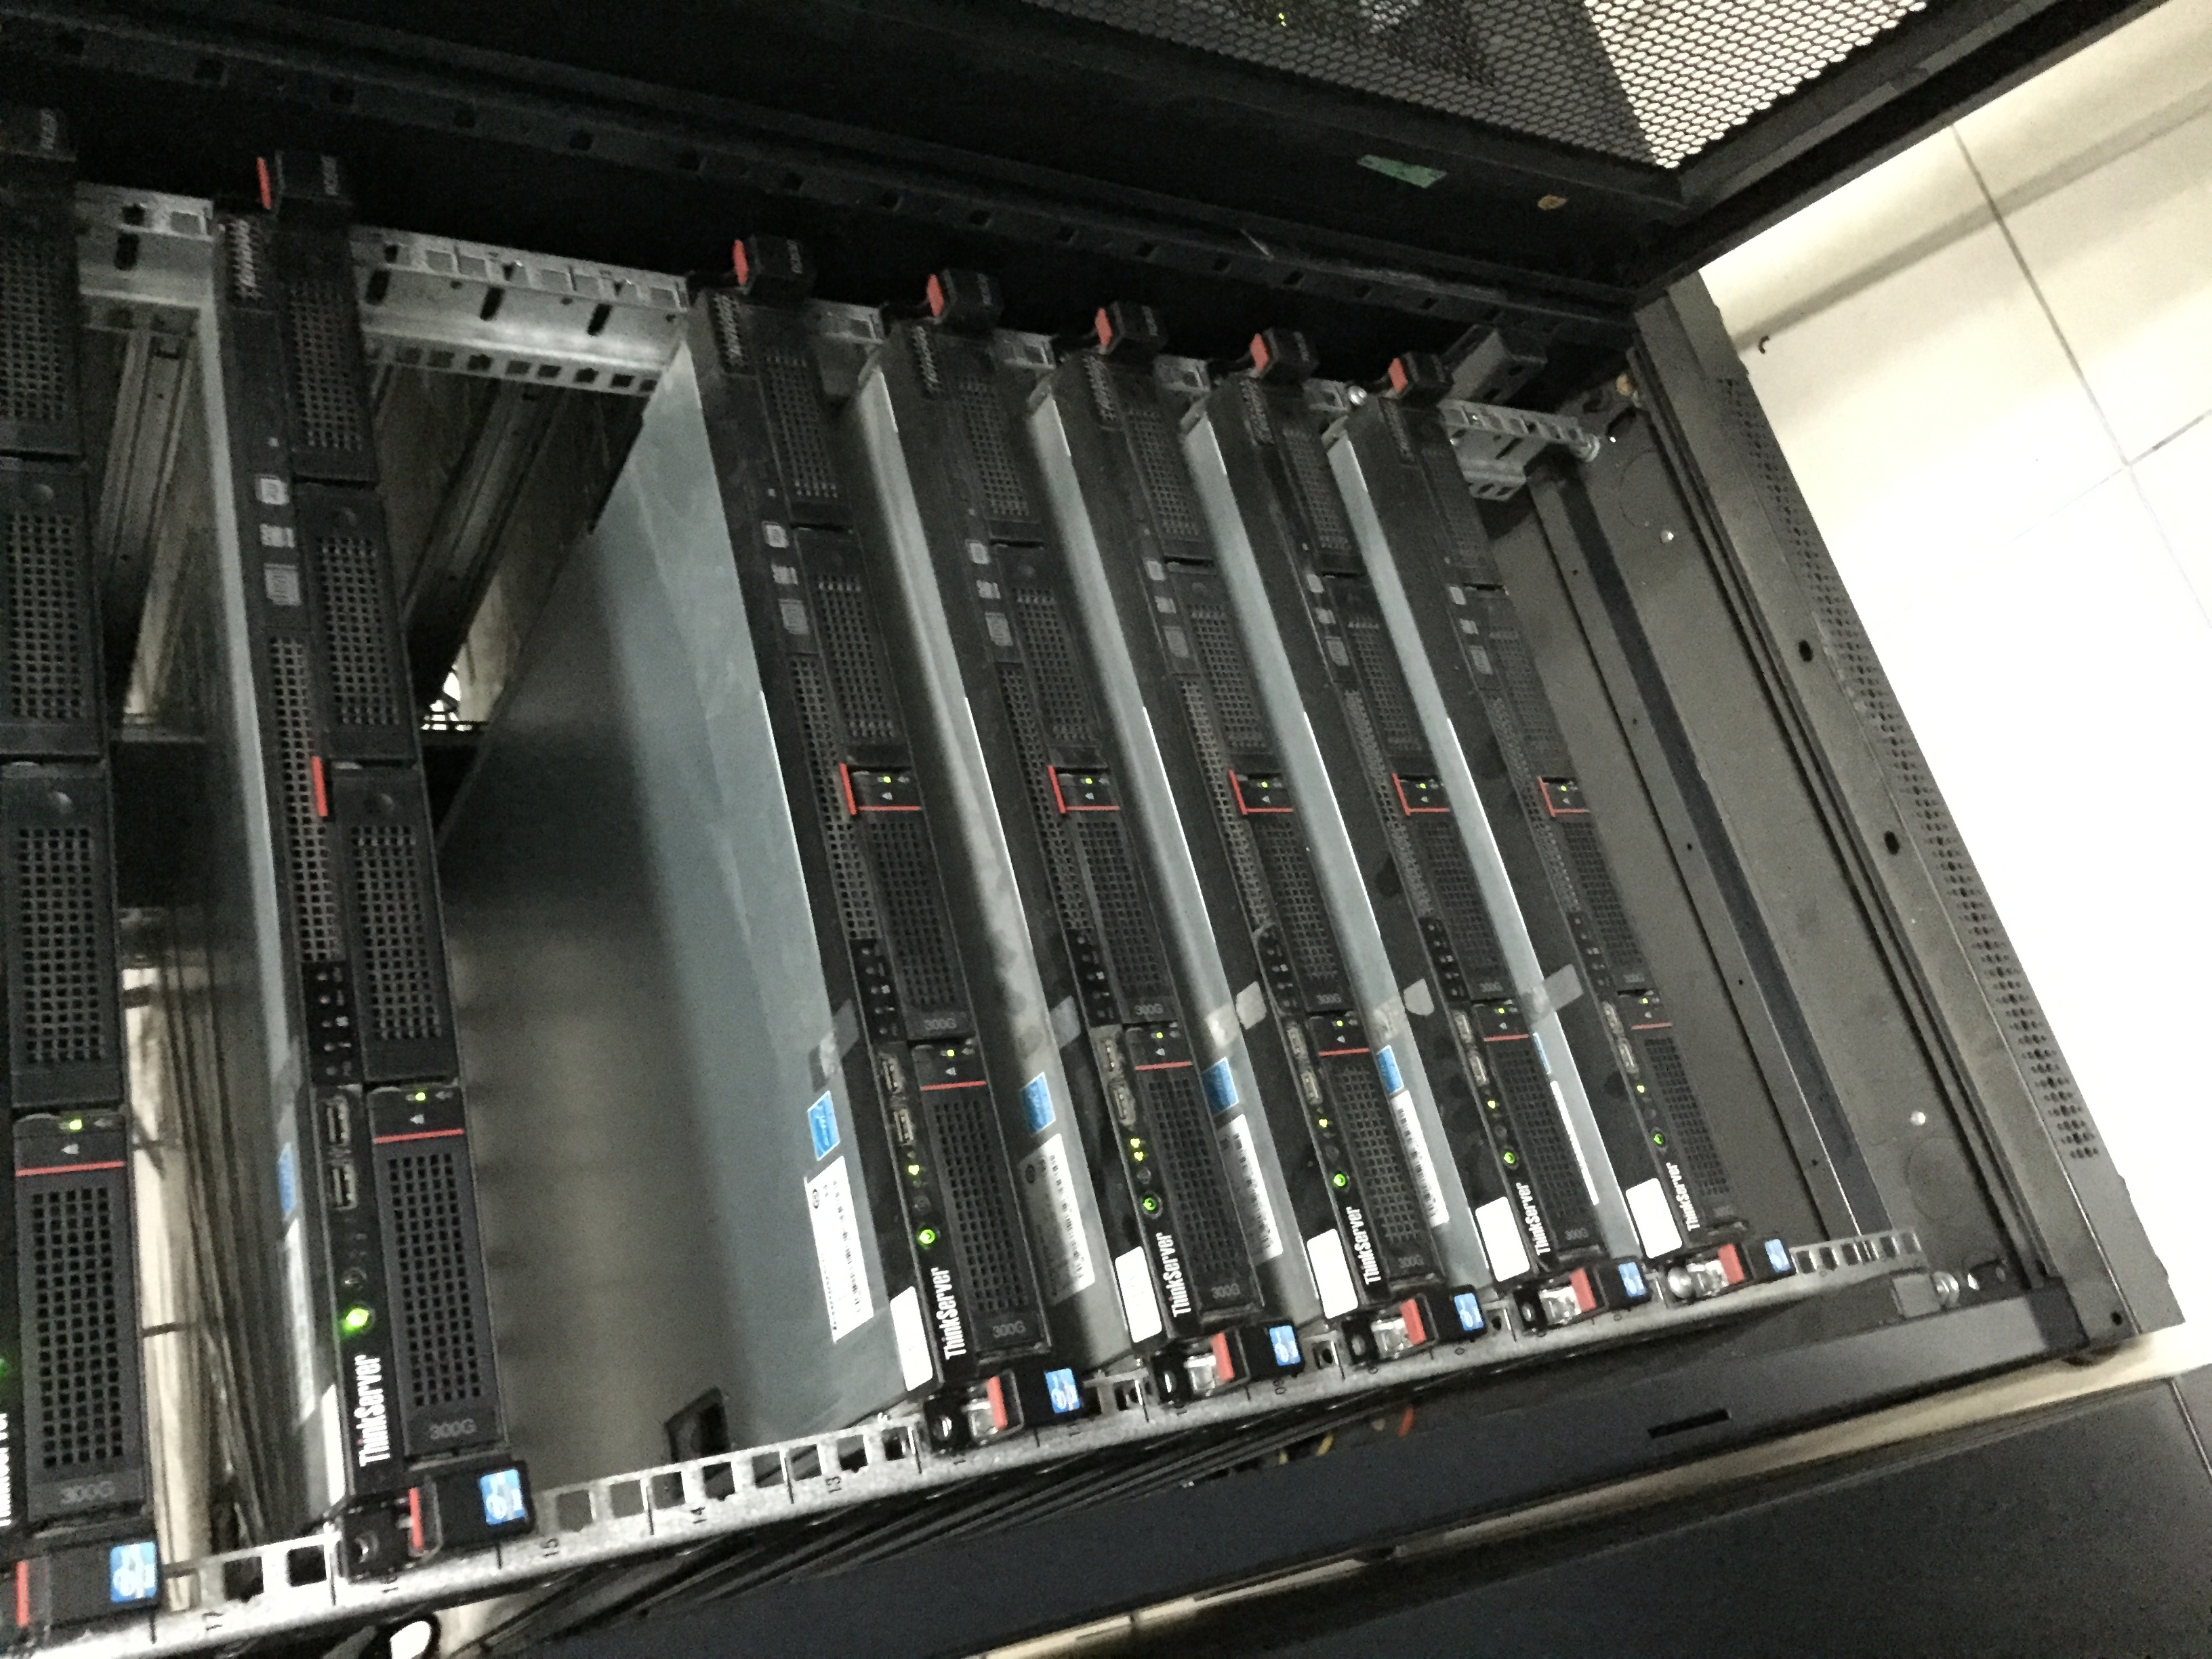
\includegraphics[height=2.5in,angle=-90]{experiment_environment1.JPG}\relax
    \let\c@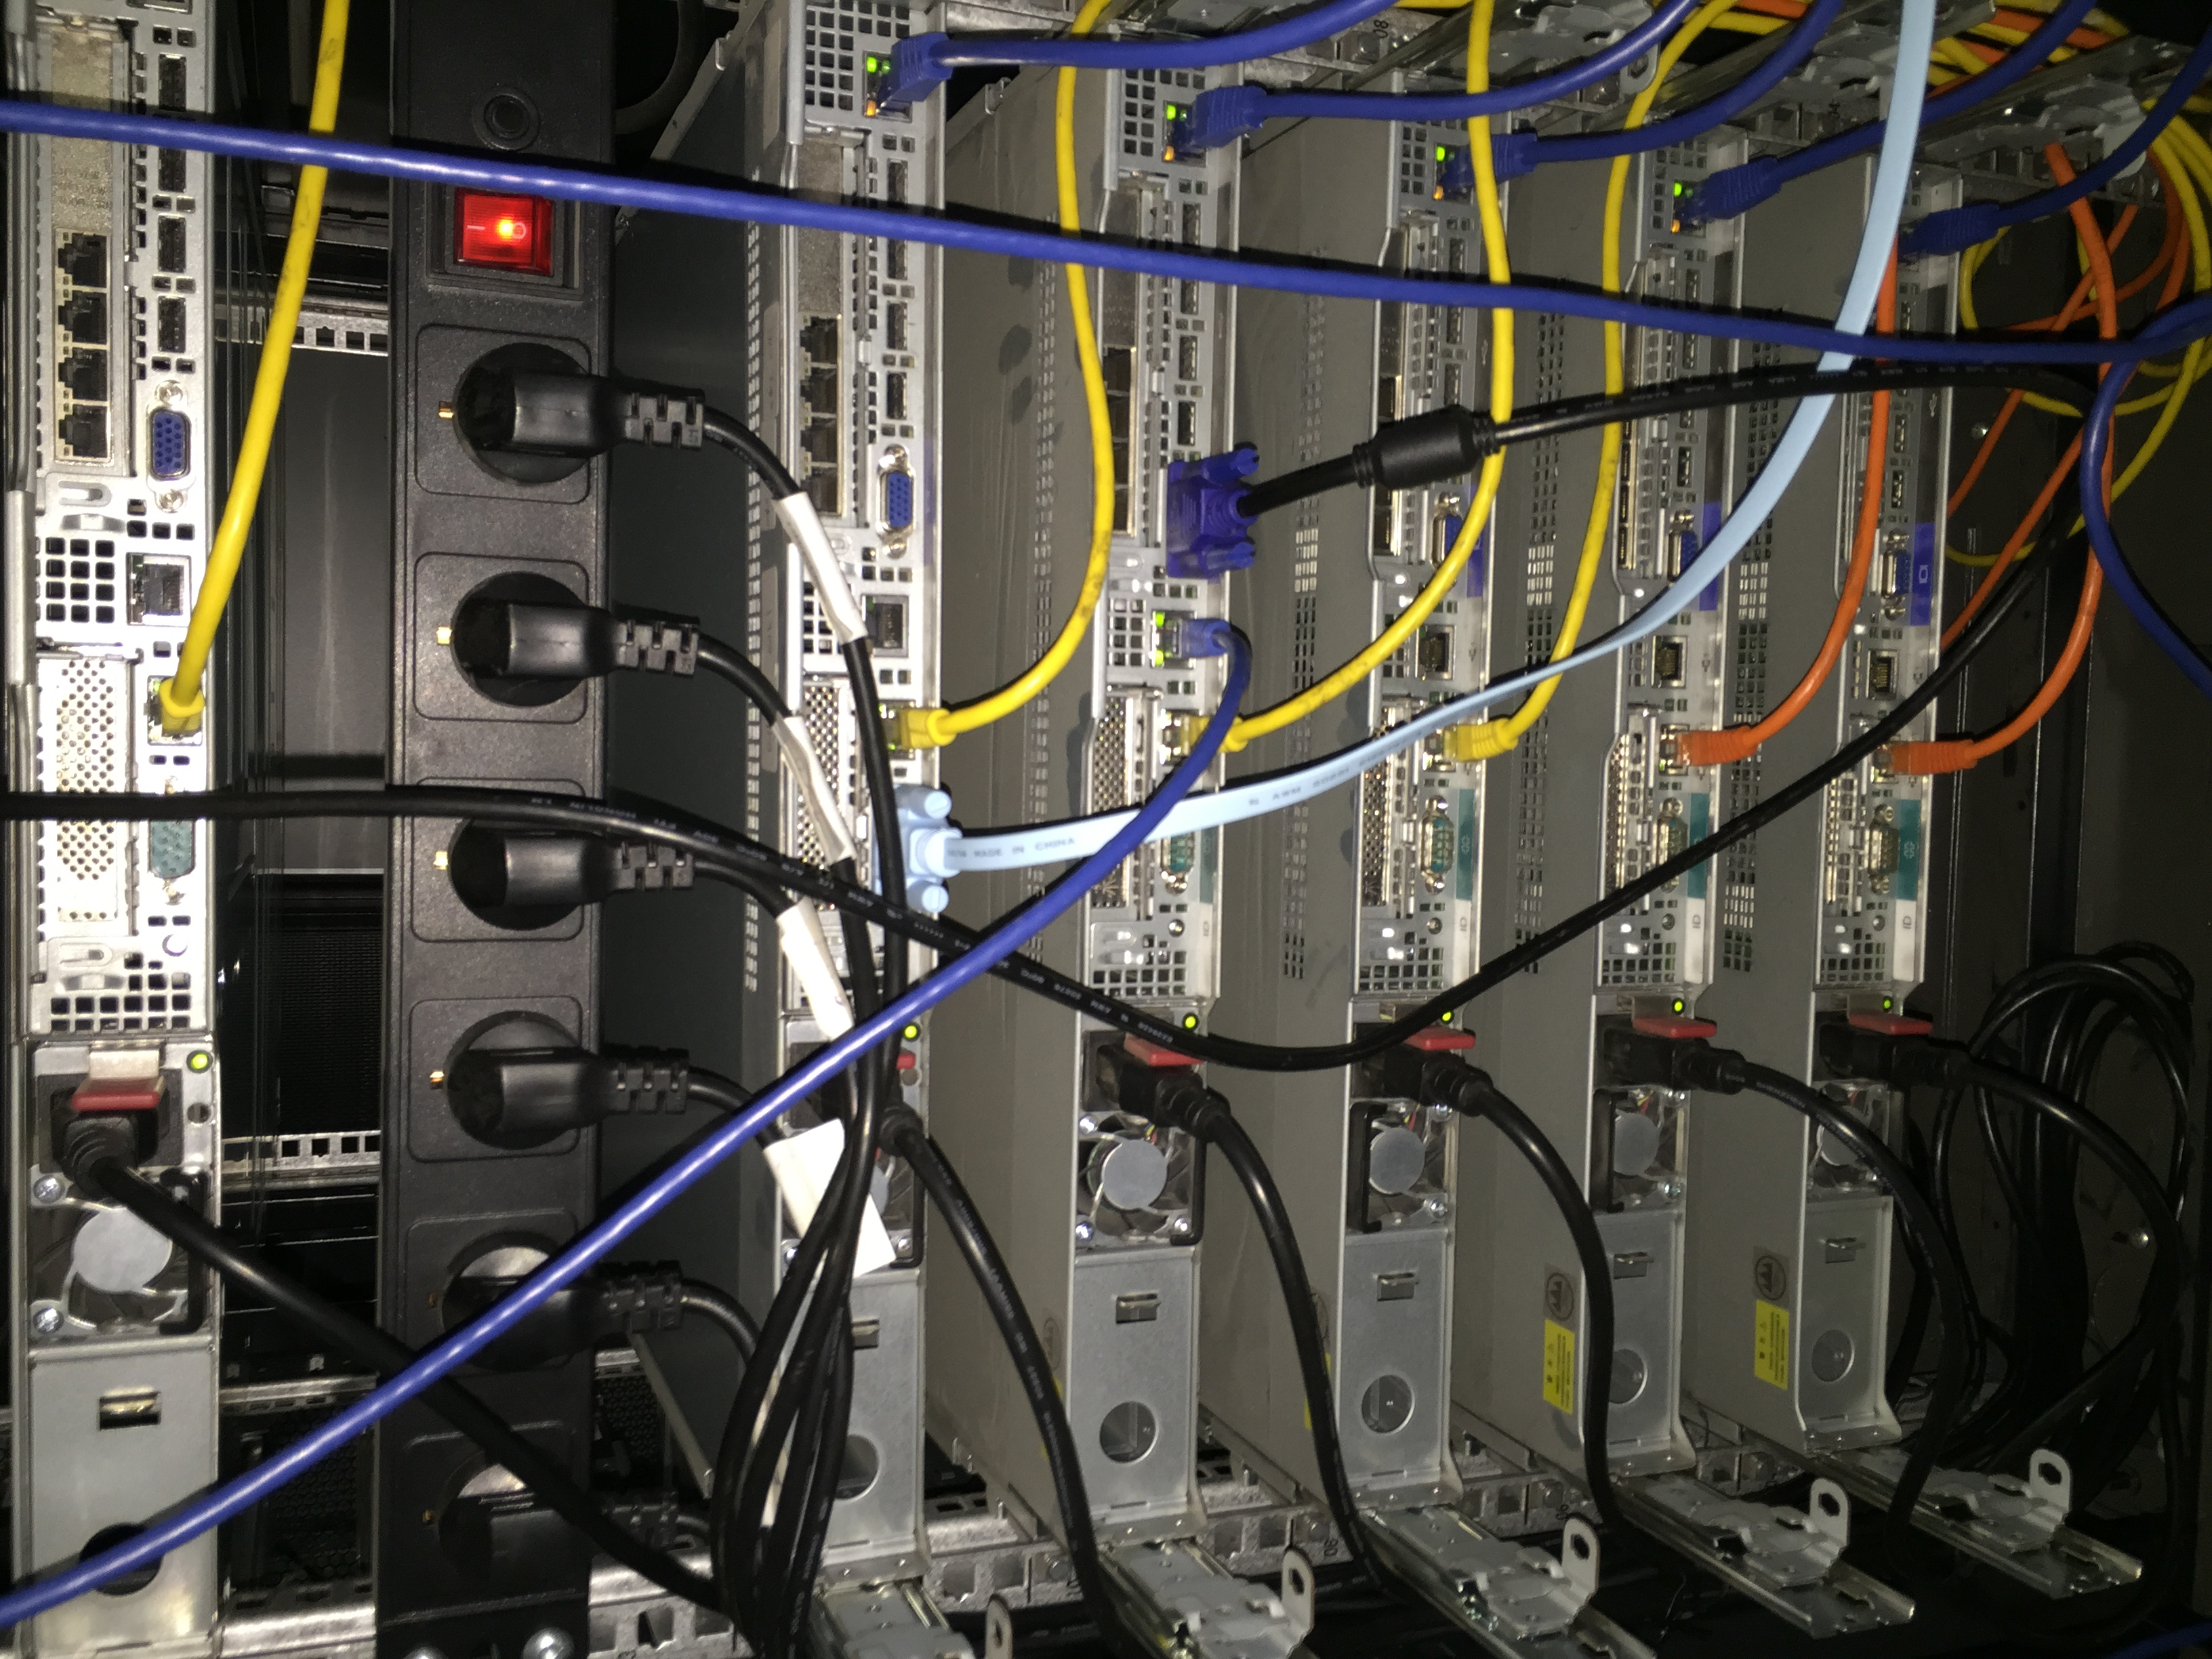
\includegraphics[height=2.5in,angle=-90]{experiment_environment2.JPG}\relax
    \caption{真实的实验环境}
\end{figure}
\subsection{实验平台搭建}
\subsubsection{Hadoop平台搭建}
搭建了hadoop平台,完成多节点的配置,进行大数据的处理
\subsubsection{SDN开发环境搭建}
搭建基于floodlight的SDN开发环境,进行网络的控制;\\

将多个虚拟交换机ovs挂载到了floodlight控制器上\\

利用ovs完成hadoop平台上的数据导流工作
\subsubsection{网络拓扑}
\begin{figure}[!htb]
    \centering
    \let\c@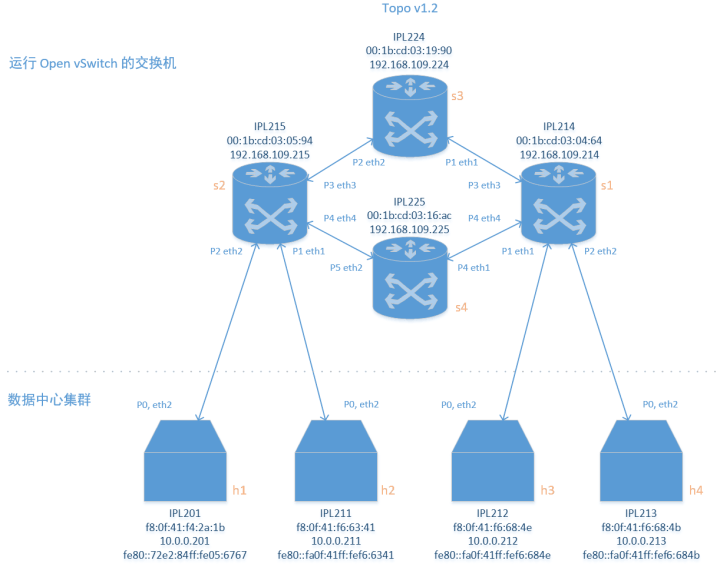
\includegraphics[height=3.5in]{topology.png}\relax
    \caption{网络拓扑结构}
\end{figure}

\subsection{coflow调度算法}
介绍我们实现的coflow调度算法\\

路由算法,最短路径路由
\section{项目的成果}

\section{项目总结}
(1).当前coflow中所有的flow都是同时出现的。考虑到实际MR中task的启动时间、map完成时间都是不相同不确定的,带来的现实情况是coflow中的flow 很大可能是不同时出现的。所以我们想采用simulator完成简单的various-start-time-coflow调度工作
(2). 将上述工作用varys实现,并采用ovs完成数据导流工作,实现整个实际平台的运行,并测试结果,对比分析。
(3).考虑更多的研究方向,如:各个coflow/flow的依赖性,除了network层面的coflow调度,把task执行联合考虑进来,例如把task尽量放到所需data的机器上。

\section{参考文献}

\bibliographystyle{plain}
\bibliography{references/reference}
%[1] J. Dean et al. MapReduce: Simplified data processing on large clusters. In OSDI, pages 137–150. 2004.\\
%[2] A. D. Ferguson et al. Participatory networking: An API for application control of SDNs. In SIGCOMM. 2013.\\
%[3] Jain S, Kumar A, Mandal S, et al. B4: Experience with a globally-deployed software defined WAN[C] ACM SIGCOMM Computer Communication Review. ACM, 2013, 43(4): 3-14.\\

%\cite{引用文章名称}
%"引用文章名称" 就是前边定义@article后面的名称.

%  \begin{figure}[!htb]
%    \centering
%\subfigure[国外]{\includegraphics[height=3in,width = 2.5in]{clipboard.png}}
%\subfigure[国内]{\includegraphics[height=3in,width = 2.5in]{Wearable.jpg}}
%        \caption{国内外监测身体状况的可穿戴设备及厂商概览}
%\end{figure}
%  \begin{figure}[!htb]
%    \centering
%    \let\c@\includegraphics[height=1.5in]{anyi.jpg}\relax
%    %\let\c@\includegraphics[height=1.2in]{fitbit.png}\relax
%        \caption{needfinding采访}
%\end{figure}
%\section{Brainstorming}
%
%%\begin{figure*}[t!]
%%    \centering
%%    \begin{subfigure}[t]{0.5\textwidth}
%%        \centering
%%        \includegraphics[height=1.2in]{iWatch.png}
%%        \caption{iWatch}
%%    \end{subfigure}%
%%    ~
%%    \begin{subfigure}[t]{0.5\textwidth}
%%        \centering
%%        \includegraphics[height=1.2in]{fitbit.png}
%%        \caption{Fitbit}
%%    \end{subfigure}
%%    \caption{腕带类可穿戴设备}
%%\end{figure*}
%\begin{figure}[!htb]
%    \centering
%    \let\c@\includegraphics[height=1.2in]{iWatch.png}\relax
%    \let\c@\includegraphics[height=1.2in]{fitbit.png}\relax
%        \caption{iWatch and Fitbit}
%\end{figure}


%\begin{figure}[!htb]
%  \centering
%  % Requires \usepackage{graphicx}
%  \includegraphics[width=1.0\textwidth]{objective-function.eps}\\
%  \caption{objective function}\label{eps:o_f}
%\end{figure}
%\begin{figure}[!htb]
%  \centering
%  % Requires \usepackage{graphicx}
%  \includegraphics[width=1.0\textwidth]{classification-Error.eps}\\
%  \caption{classification Error}\label{eps:classification-Error}
%\end{figure}

%%%%%%%%%%  参考文献  %%%%%%%%%%

\clearpage
\end{CJK*}                                     % 结束中文字体使用
\end{document}                                 % 结束全文
